% Краткая постановка; компилировать XeLaTeX. Подробности в main.tex.
\documentclass[aspectratio=169,11pt]{beamer}
\usepackage{fontspec}
\setmainfont{DejaVuSerif.ttf}[Path=fonts/,BoldFont=DejaVuSerif-Bold.ttf]
\setsansfont{DejaVuSerif.ttf}[Path=fonts/,BoldFont=DejaVuSerif-Bold.ttf]
\usepackage[russian]{babel}
\usepackage{amsmath,amssymb}
\usetheme{default}
\usecolortheme{dove}
\setbeamertemplate{navigation symbols}{}
\setbeamertemplate{footline}[frame number]
\setbeamercolor{frametitle}{fg=blue!55!black}
\newcommand{\CE}{\operatorname{CE}}
\newcommand{\NII}{\operatorname{NII}}
\newcommand{\MtM}{\operatorname{MtM}}
\newcommand{\E}{\mathbb E}
\newcommand{\Pp}{\mathbb P}
\newcommand{\Qq}{\mathbb Q}
\begin{document}

\begin{frame}{1. Баланс и состояние в абсолютных величинах}
\begin{block}{Баланс банка}
\[
L_t=F_t+(L_t-F_t),\qquad D_t=\nu L_t,\qquad C_t=E_t+D_t-L_t.
\]
\end{block}
\begin{description}
\item[$L_t$] общий остаток кредитов: fixed $F_t$ и float $L_t-F_t$;
\item[$D_t$] депозиты; $\nu>0$ --- заданное отношение депозитов к кредитам;
\item[$E_t$] бухгалтерский капитал; $C_t$ --- денежная позиция, которая может быть отрицательной.
\end{description}
\medskip
\textbf{Полное состояние} $(L_t,X_t)$, где $X_t=(r_t,F_t,Y_t,E_t)$.
Здесь $r_t$ --- короткая ставка, а $Y_t$ --- сумма годовых купонов
старых fixed-кредитов и \emph{договорных спредов} старых float-кредитов.
Агрегат $Y_t$ хранит эффект прошлых выдач без отдельного учёта каждого винтажа.
\end{frame}

\begin{frame}{2. Управление, рост книги и новая выдача}
\textbf{Управление} $f_t\in[0,1]$ --- доля \emph{новой выдачи} в fixed-кредитах.
Доля float равна $1-f_t$. Уже накопленная доля fixed равна $F_t/L_t$.
\medskip

Каждый кредит амортизируется с интенсивностью $\mu$.
Поток новой выдачи зависит от текущей ставки:
\[
I_t=(\mu+g_0)e^{-\chi(r_t-r_0)}L_t,
\qquad g(r_t)=I_t/L_t-\mu.
\]
Чистое изменение остатка книги:
\[
\underbrace{dL_t}_{\text{изменение остатка}}
=\underbrace{-\mu L_t\,dt}_{\text{погашения}}
+\underbrace{I_t\,dt}_{\text{новая выдача}}
=g(r_t)L_t\,dt.
\]
То есть новая выдача должна компенсировать выгашывание текущих кредитов и обеспечивать рост книги, который зависит от ставки.

Fixed-выдача равна $f_tI_t$, float-выдача --- $(1-f_t)I_t$.
\medskip

\footnotesize
$g_0$ --- рост при $r_0$; $\chi$ --- чувствительность выдачи к ставке.
При $\chi=0$ получаем детерминированный рост $L_t=L_0e^{g_0t}$.
\end{frame}

\begin{frame}{3. Ставки новых кредитов}
Под мерой ценообразования $\Qq$ определим цену единицы платежа
через $u$ лет при текущей ставке $r$:
\[
P_Q(r,u)=\E_r^{\Qq}\!\left[
\exp\!\left(-\int_0^u r_s\,ds\right)\right],
\qquad
A_Q(r)=\int_0^\infty e^{-\mu u}P_Q(r,u)\,du.
\]
$A_Q(r)$ --- приведённая стоимость потока единичных платежей,
уменьшающегося вместе с остатком амортизируемого кредита.
\begin{align*}
\text{Новый fixed:}\quad k_F(r)&=A_Q(r)^{-1}-\mu+s_F,\\
\text{Новый float:}\quad r_t+s_V(1-f_t),\qquad
s_V(q)&=s_V^0-\eta q.
\end{align*}
\footnotesize
$A_Q^{-1}-\mu$ --- par-купон: приведённая стоимость купона и погашения
основного долга равна номиналу. $s_F$ и $s_V^0$ --- продуктовые надбавки;
в текущей калибровке $s_F=s_V^0$.

$\eta$ снижает маржу при росте доли float в новой выдаче.
\end{frame}

\begin{frame}{4. Динамика ставки и кредитной книги}
Под физической мерой $\Pp$ ставка следует CIR-процессу:
\[
dr_t=\kappa_P(\bar r_P-r_t)\,dt
+\sigma\sqrt{r_t}\,dW_t^{\Pp}.
\]
Остаток fixed-кредитов и агрегат договорных платежей меняются так:
\begin{align*}
dF_t&=\bigl[I_tf_t-\mu F_t\bigr]dt,\\[0.5em]
dY_t&=\Bigl[I_t
\bigl\{f_tk_F(r_t)+(1-f_t)s_V(1-f_t)\bigr\}
-\mu Y_t\Bigr]dt.
\end{align*}
\footnotesize
В $Y_t$ добавляются купон нового fixed-кредита и спред нового
float-кредита. Текущая базовая ставка $r_t$ по float-кредитам в
$Y_t$ не фиксируется. Параметры $\kappa_P,\bar r_P,\sigma$
описывают фактическую динамику рыночной ставки.
\end{frame}

\begin{frame}{5. Процентный доход, прибыль и капитал}
\small
\begin{align*}
n_t={}&
\underbrace{Y_t}_{\text{старые купоны и спреды}}
+\underbrace{r_t(L_t-F_t)}_{\text{базовая ставка float}}
+\underbrace{r_tC_t}_{\text{денежная позиция}}\\
&-\underbrace{(\beta r_t+s_D)D_t}_{\text{стоимость депозитов}}
-\underbrace{s_B(-C_t)^+}_{\text{дорогое финансирование}},\\[0.4em]
\Pi_t={}&n_t-\underbrace{\omega D_t}_{\text{операционные расходы}},\\[0.4em]
dE_t={}&(1-\alpha)\Pi_t\,dt.
\end{align*}
\medskip
Владельцу выплачивается $\alpha\Pi_t\,dt$ в виде дивидендов. Доля $1-\alpha$ остаётся в капитале.
Жёсткого ограничения на капитал нет.
\end{frame}

\begin{frame}{6. Функционал оптимального управления}
\small
Для численного решения нормируем $F,Y,E$ на $L_t$:
состояние становится $(r,F/L,Y/L,E/L)$.

Ищем \emph{стационарную} политику обратной связи
$f_t=\pi(r_t,F_t/L_t,Y_t/L_t,E_t/L_t)\in[0,1]$,
максимизирующую риск-чувствительную стоимость \emph{всего будущего}
потока $\alpha\Pi_t\,dt$ владельцу.
Для случайной величины $Z$:
\[
\CE_\gamma(Z\mid X)
=-\gamma^{-1}\log\E^{\Pp}[e^{-\gamma Z}\mid X],
\qquad \gamma_t=\bar\gamma/L_t.
\]
Для \emph{заданной} политики $\pi$ определим её оценку обратно
от конечного горизонта $T$, где $J_T^\pi(T,L,X)=0$:
\[
J_T^\pi(t,L,X)=B_{t,t+h}^{\mathrm{PV}}(L,X,\pi)
+e^{-r_th}\CE_{\gamma_t}\!\left(
J_T^\pi(t+h,L_{t+h},X_{t+h})\mid L_t=L,X_t=X,\pi\right).
\]
\[
\boxed{\displaystyle V(L,X)=\sup_\pi\lim_{T\to\infty}J_T^\pi(t,L,X).}
\]
\footnotesize
$B_{t,t+h}^{\mathrm{PV}}$ --- поток $\alpha\Pi_s\,ds$,
дисконтированный внутри шага по рыночной ставке.
Это рекурсивный критерий; терминальной награды нет.
При случайном росте стоимость в абсолютных величинах зависит от
текущего $L_t$; правило $\pi$ явного времени не содержит.
\end{frame}

\begin{frame}{7. Замороженный баланс: $\NII_{1y}$ и его шок}
\small
В текущем состоянии фиксируем $L,D,F,Y,E,C$ на следующий год:
нет погашений, новой выдачи и управления.
Сравниваем постоянную ставку $r$ со ставкой $r+\delta$,
$\delta=0.01$ (100 б.п.).
\begin{align*}
\NII_{1y}(r)={}&
\bigl[Y+r(L-F)+rC-(\beta r+s_D)D-s_B(-C)^+\bigr]
\cdot1\text{ год},\\[0.6em]
\Delta\NII_{1y}={}&\NII_{1y}(r+\delta)-\NII_{1y}(r)\\
={}&\delta\underbrace{\bigl[(L-F)+C-\beta D\bigr]}_{
\text{переоцениваемый объём}}\cdot1\text{ год}.
\end{align*}
\footnotesize
Рост ставки повышает доход по float-остатку $L-F$,
меняет результат денежной позиции на $C$ (при $C<0$ это расход)
и увеличивает стоимость депозитов на $\beta D$.
Купоны fixed и спреды в $Y$ не меняются.
При прочих равных большая доля fixed уменьшает чувствительность
$\Delta\NII_{1y}$.
\end{frame}

\begin{frame}{8. Рыночная стоимость: $\MtM$ и её шок}
\small
При переоценке \emph{существующего} баланса float-номинал и депозиты
принимаем равными номиналу, а фиксированные договорные платежи
дисконтируем по кривой $Q$:
\begin{align*}
\MtM(r)
&=\underbrace{C+(L-F)-D}_{\text{cash, float, депозиты по номиналу}}
+\underbrace{(Y+\mu F)A_Q(r)}_{
\text{купоны, спреды и возврат fixed-номинала}}\\
&=E-F+(Y+\mu F)A_Q(r),\\[0.6em]
\Delta\MtM
&=\MtM(r+\delta)-\MtM(r)\\
&=(Y+\mu F)\bigl[A_Q(r+\delta)-A_Q(r)\bigr].
\end{align*}
\footnotesize
$A_Q(r)$ убывает со ставкой, поэтому при $Y+\mu F>0$ шок вверх
даёт $\Delta\MtM<0$. $Y$ включает также зафиксированные спреды float.
Чем больше фиксированных будущих платежей, тем сильнее переоценка.
В отличие от $\Delta\NII_{1y}$,
здесь учитываются платежи за пределами одного года.
\medskip
\end{frame}

\begin{frame}{9. Один шок, три разных риск-метрики}
\centering
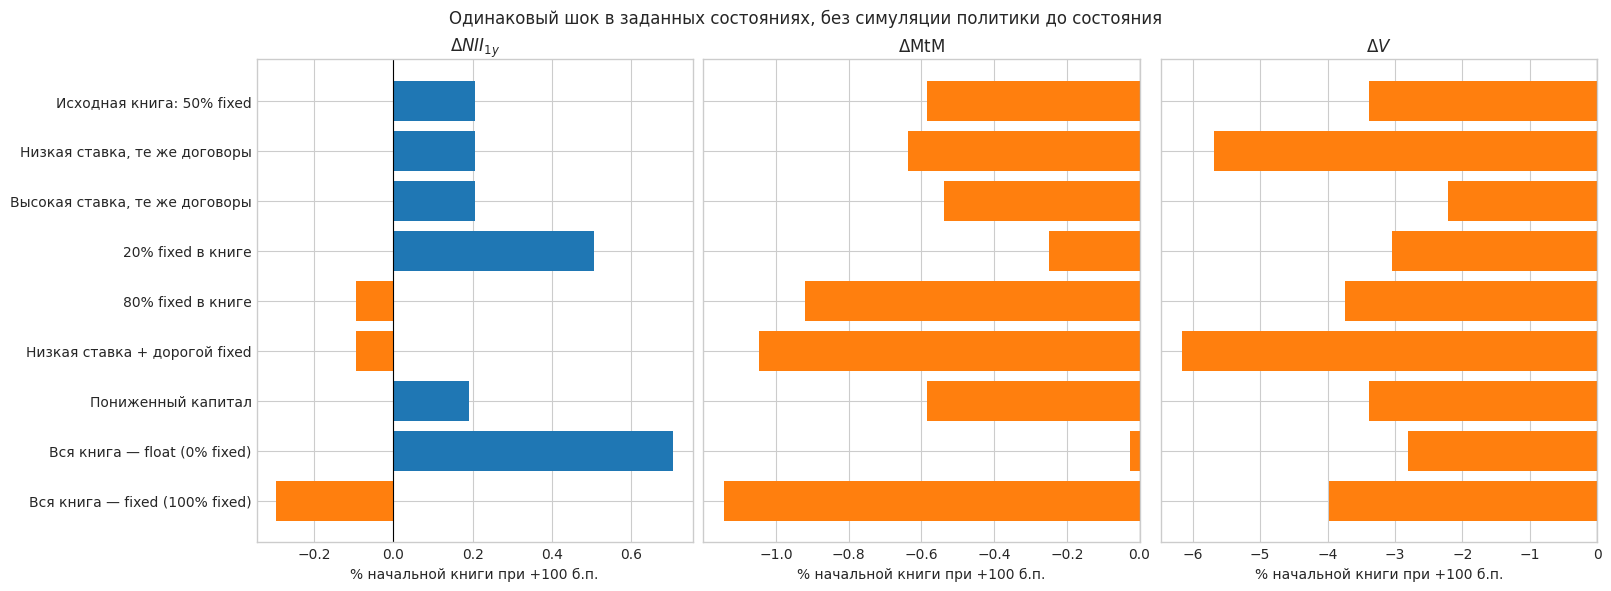
\includegraphics[width=\textwidth,height=.70\textheight,keepaspectratio]{figures/risk_03.png}
\par\smallskip
\begin{minipage}{.96\textwidth}\scriptsize
Во всех сценариях ставка немедленно повышается на 100 б.п., далее обе траектории ставки получают одинаковые случайные приращения; состояние до шока задано вручную.
$\Delta\NII_{1y}$ относится к годовому горизонту (баланс считаем замороженным), $\Delta\MtM$ --- к старым договорам,
$\Delta V$ --- к будущим выплатам дивидендов при дальнейшей обратной связи.
Все три величины на рисунке выражены как доля начальной книги, но относятся к разным горизонтам.
\end{minipage}
\end{frame}

\begin{frame}{10. Почему меняется $\Delta\NII_{1y}$}
\small
\[
\Delta\NII_{1y}=\delta\underbrace{(L-F)}_{\text{плавающие кредиты}}
+\delta\underbrace{C}_{\text{денежная позиция}}
-\delta\underbrace{\beta D}_{\text{депозиты}},\qquad\delta=0.01 \text{ -- шок ставки}.
\]
\centering
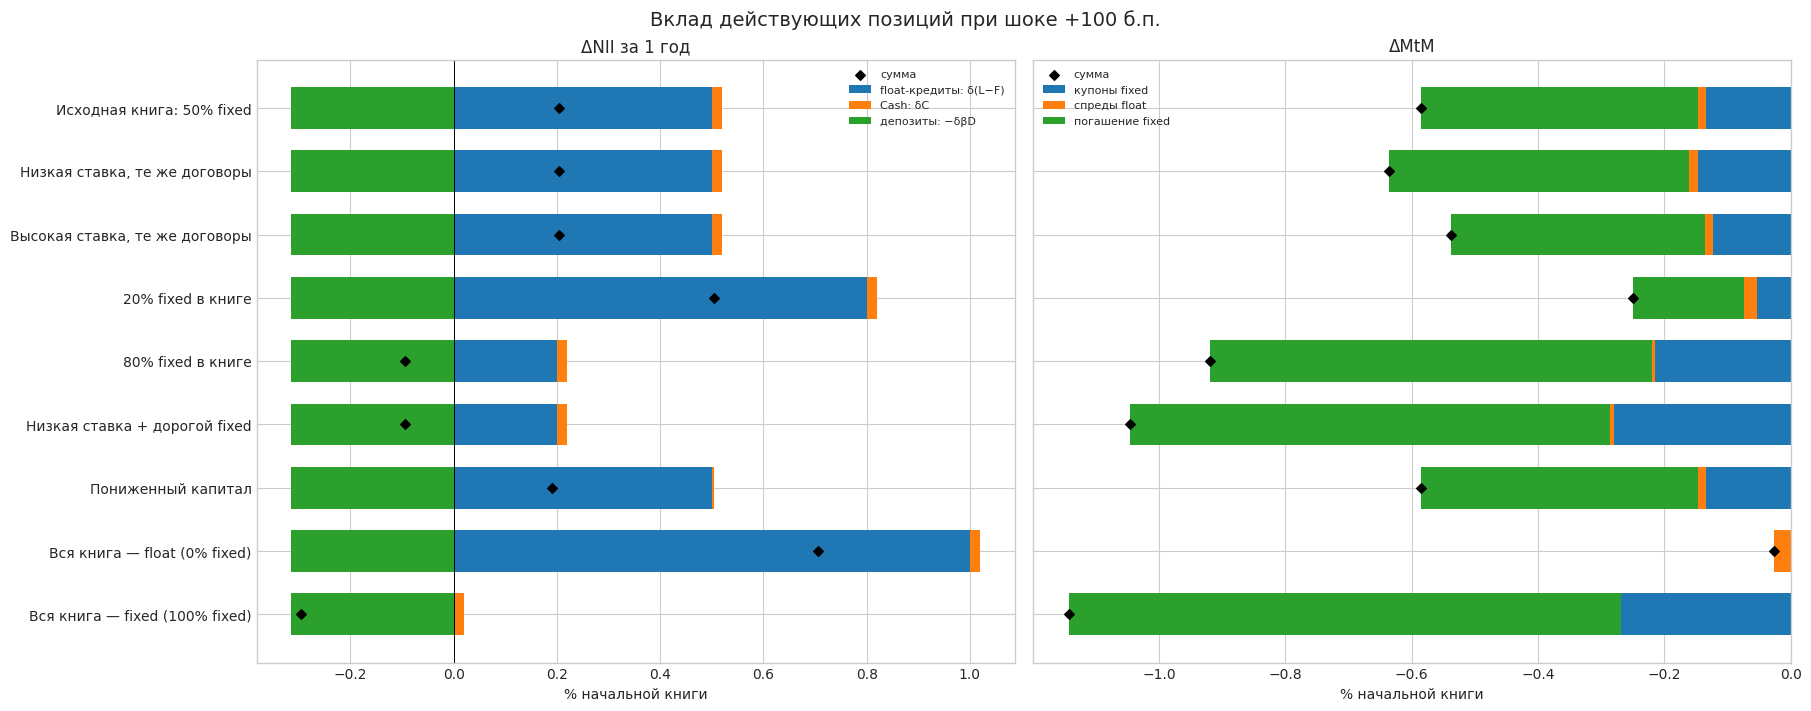
\includegraphics[width=\textwidth,height=.56\textheight,keepaspectratio]{figures/risk_05.png}
\par\vspace{-.5ex}
\begin{minipage}{.96\textwidth}\scriptsize
Левая панель: вклад float растёт при снижении доли fixed; вклад депозитов одинаков,
так как во всех показанных состояниях $L=L_0$ и $D=\nu L_0$.
Вклад $C$ мал при выбранном начальном балансе. Чёрный ромб --- сумма трёх вкладов.
Правая панель понадобится для $\Delta\MtM$ на следующем слайде.
\end{minipage}
\end{frame}

\begin{frame}{11. Почему меняется $\Delta\MtM$}
\small
\[
\Delta\MtM=(Y+\mu F)\Delta A_Q,
\qquad \Delta A_Q=A_Q(r+\delta)-A_Q(r)<0.
\]
\centering
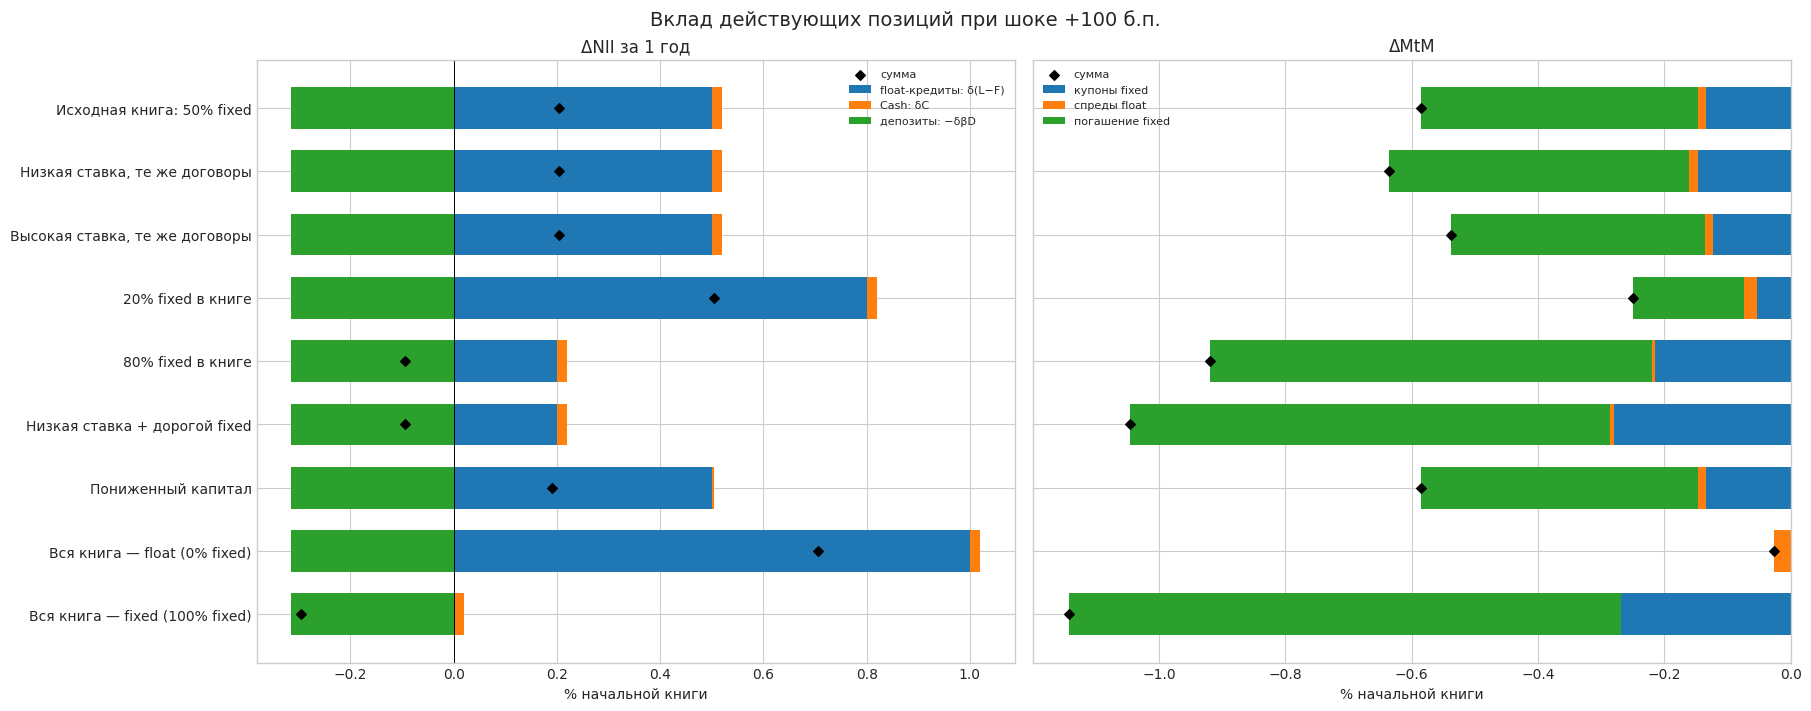
\includegraphics[width=\textwidth,height=.56\textheight,keepaspectratio]{figures/risk_05.png}
\par\vspace{-.5ex}
\begin{minipage}{.96\textwidth}\scriptsize
Правая панель: $Y$ распадается на купоны старых fixed и спреды старых float;
$\mu F$ --- поток погашения fixed-основной суммы. Их сумма умножается на
отрицательное $\Delta A_Q$. Поэтому увеличение fixed усиливает убыток от шока.
Левая панель показывает противоположное направление зависимости $\Delta\NII_{1y}$.
\end{minipage}
\end{frame}

\begin{frame}{12. Что сравнивает парный эксперимент}
\small
Хотим понять, чем вызвано сильное различие метрик $\Delta MtM$ и $\Delta V$ в абсолютных значениях.
Исходное состояние: $r=8\%$, $F/L=50\%$, $E/L=12\%$.
Во второй ветви меняется только начальная ставка: $8\%\mapsto9\%$.
В дальнейшем обе ветви получают одинаковые случайные приращения.
\medskip

Для каждого шага $k$ дисконтированная дивидендная выплата владельцу представлена как
\[
PV_k=\mathcal D_k L_{k+1/2}m_k,
\]
где $\mathcal D_k$ --- накопленный и внутришаговый дисконт-фактор,
$L_{k+1/2}$ --- размер книги,
$m_k$ --- выплата за шаг на единицу книги.
% Сравниваем либо постоянную выдачу $f=50\%$, либо обученную обратную связь.
\medskip

\begin{block}{Точное разложение разности на каждом шаге}
\scriptsize
\[
\Delta PV_k=
\underbrace{(\mathcal D_k^{+1\%}-\mathcal D_k)L_{k+1/2}m_k}_{\text{дисконт}}
+\underbrace{\mathcal D_k^{+1\%}(L_{k+1/2}^{+1\%}-L_{k+1/2})m_k}_{\text{размер книги}}
+\underbrace{\mathcal D_k^{+1\%}L_{k+1/2}^{+1\%}(m_k^{+1\%}-m_k)}_{\text{выплата на единицу книги}}.
\]
\end{block}
\end{frame}

% \begin{frame}{13. Парный шок: постоянная выдача 50\% fixed}
% \centering
% 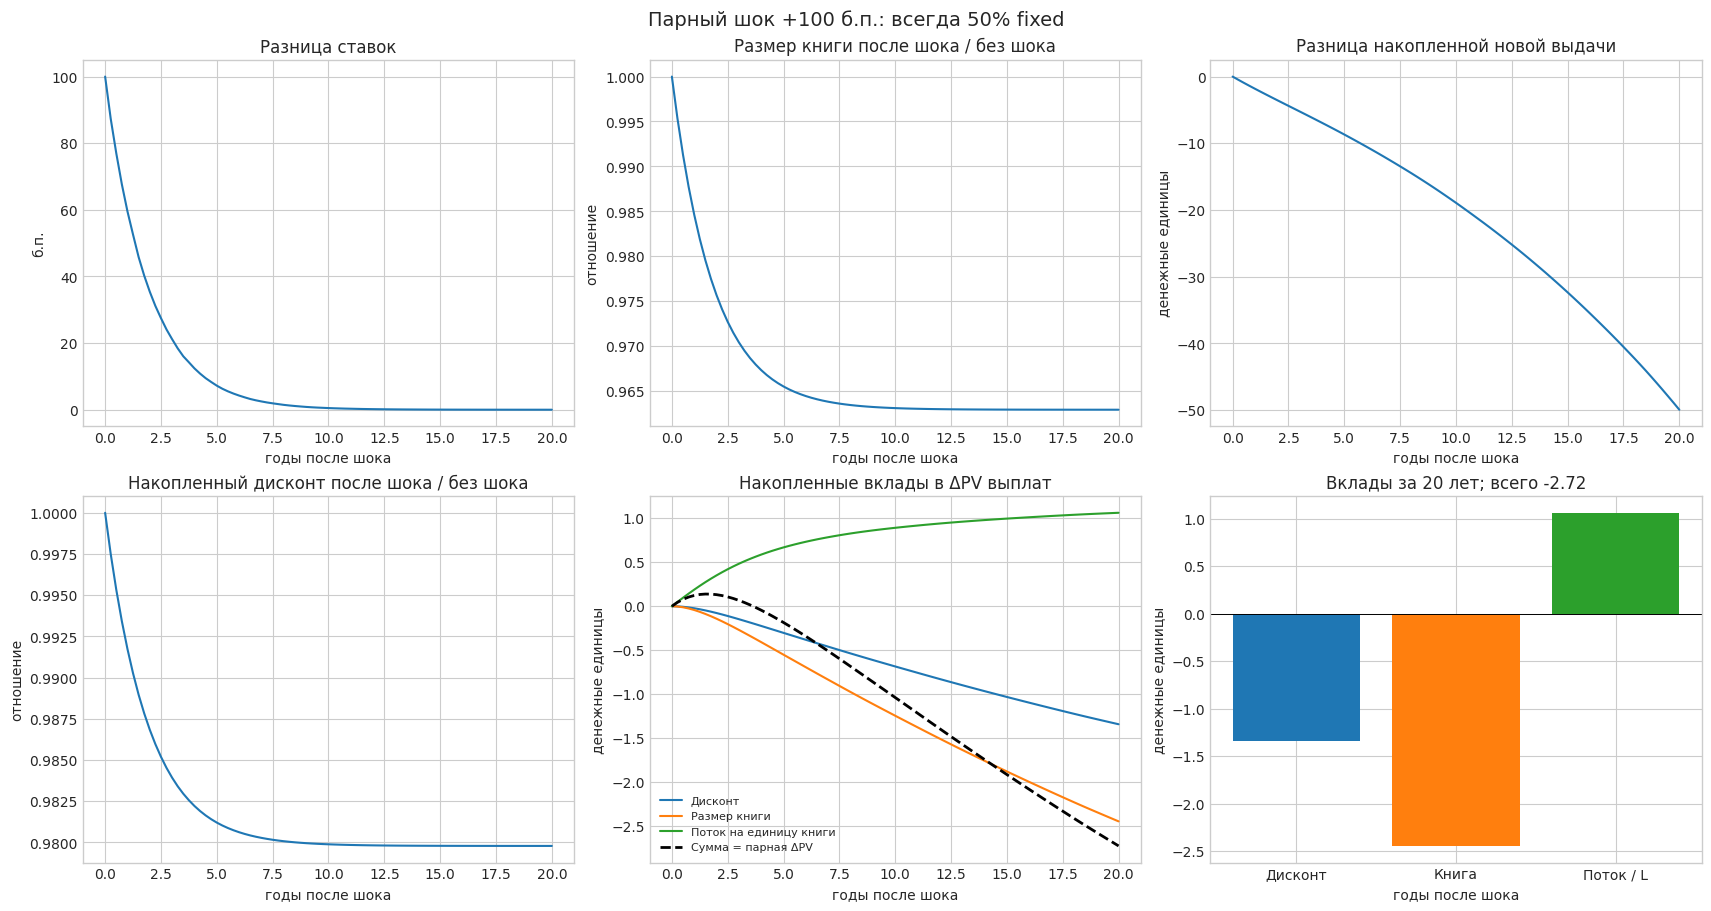
\includegraphics[width=\textwidth,height=.88\textheight,keepaspectratio]{figures/risk_07.png}
% \end{frame}

\begin{frame}{13. Парный шок: обученная обратная связь}
\centering
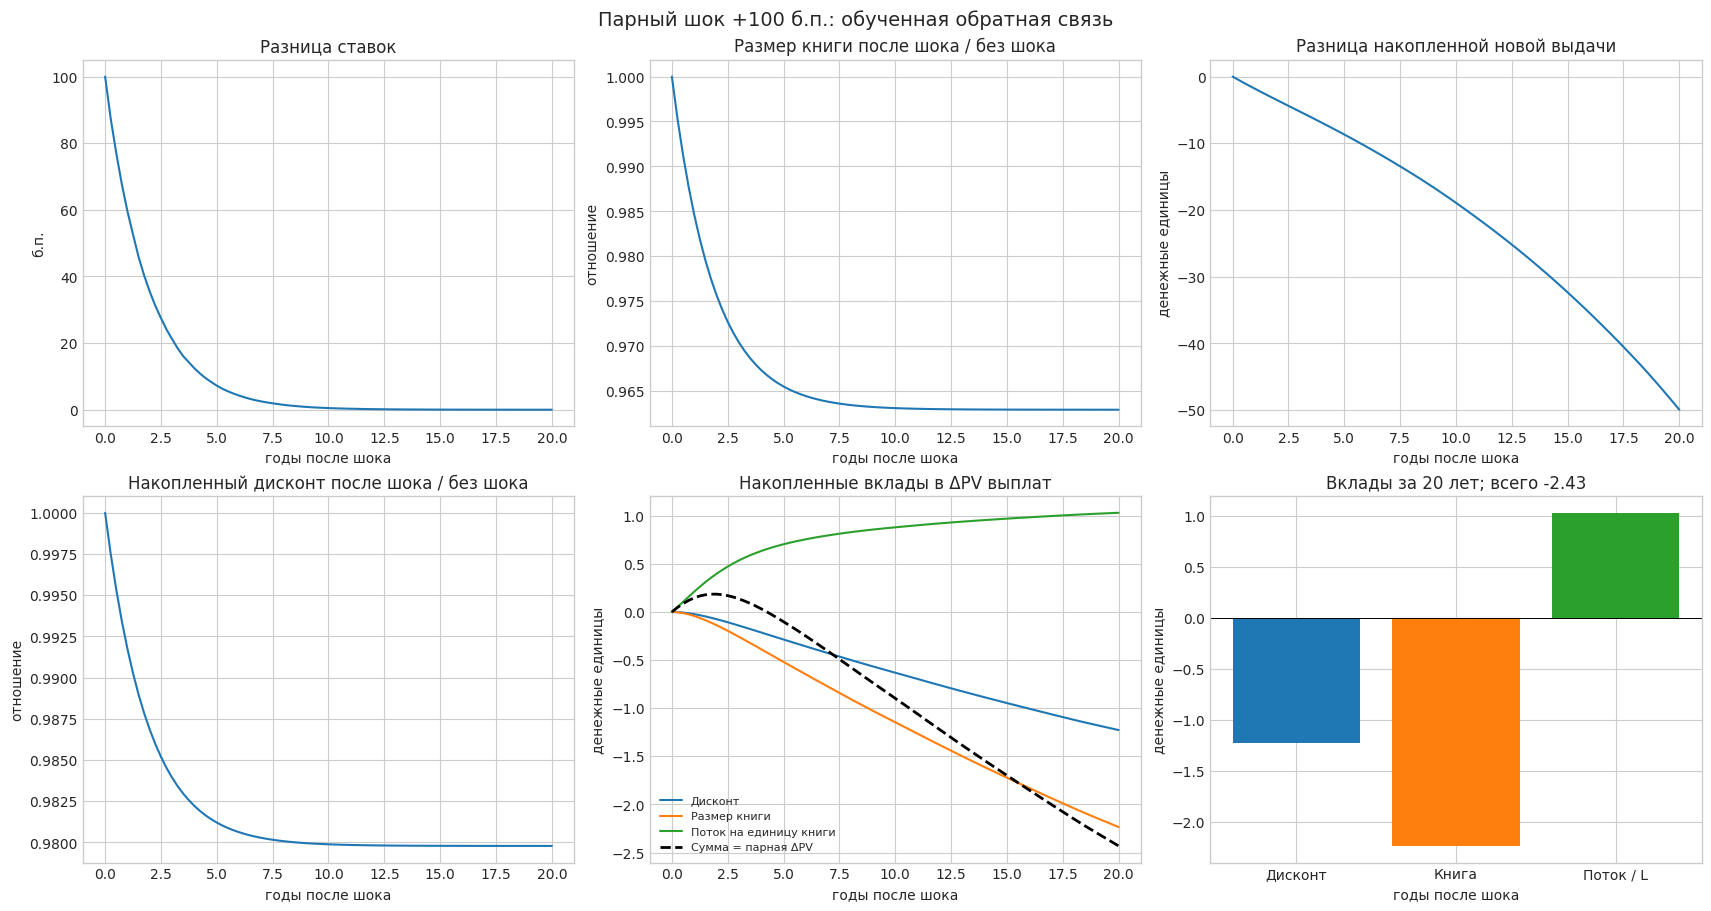
\includegraphics[width=\textwidth,height=.88\textheight,keepaspectratio]{figures/risk_09.png}
\end{frame}

\begin{frame}{14. Интерпретация парного $\Delta PV$}
\small
В численной схеме валовая выдача за шаг равна
\[
I_k=L_{k+1}-e^{-\mu h}L_k,
\qquad B_t=\exp\!\left(-\int_0^t r_s\,ds\right).
\]
На графиках показаны разность $\sum_{k<t/h}I_k^{+1\%}-\sum_{k<t/h}I_k$
и отношение накопленных дисконт-факторов $B_t^{+1\%}/B_t$.
Шок уменьшает новую выдачу и оставляет книгу примерно на 3.7\% меньше;
накопленный дисконт приблизительно на 2\% ниже.
\medskip

\begin{center}
\begin{tabular}{lrrrr}
\hline
Стратегия & дисконт & книга & поток/$L$ & сумма \\
\hline
Постоянная выдача 50\% fixed & $-1.34$ & $-2.44$ & $+1.06$ & $-2.72$ \\
Обученная & $-1.23$ & $-2.24$ & $+1.03$ & $-2.43$ \\
\hline
\end{tabular}
\end{center}
\footnotesize
Рост ставки повышает удельный поток через float-доход и cash,
но не перекрывает меньшую книгу и более сильное дисконтирование.
Это суммы дисконтированных выплат \emph{только за 20 лет}, без остаточного
капитала и без энтропийной оценки.
\end{frame}

\begin{frame}{15. Относительная чувствительность}
\centering
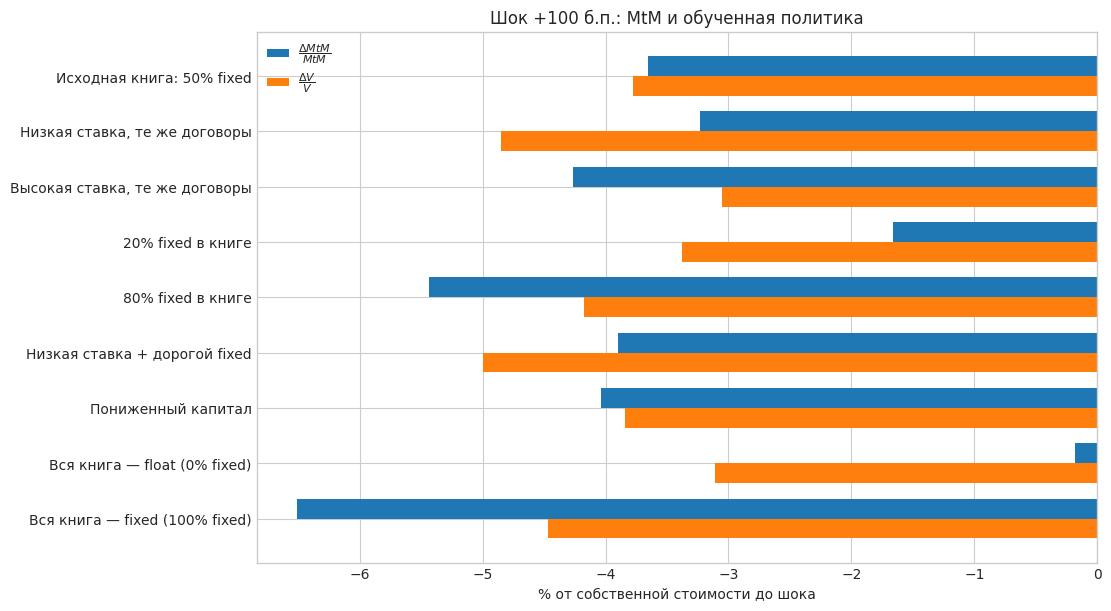
\includegraphics[width=\textwidth,height=.72\textheight,keepaspectratio]{figures/risk_16.png}
\par\smallskip
\begin{minipage}{.96\textwidth}\scriptsize
Знаменатели --- собственные значения метрик \emph{до} шока: $\Delta\MtM/\MtM$
и $\Delta V/V$. В исходном состоянии проценты близки, несмотря на большую
разницу денежных дельт. Это не универсально: при полностью плавающей книге
$\Delta\MtM$ почти нулевая, а $\Delta V$ остаётся отрицательной.
\end{minipage}
\end{frame}

\begin{frame}{16. Разложение $\Delta V$}
\small
Пусть $J_\gamma^\pi$ --- бессрочная стоимость политики $\pi$
при риск-чувствительности $\gamma$, $\widehat\pi$ --- обученная
обратная связь, $\widehat V$ --- выход обученной сети.
Для любой величины $H$ обозначим $\Delta H=H(x^{+1\%})-H(x)$.
\medskip
\begin{align*}
\Delta\widehat V={}&\underbrace{\Delta\MtM}_{\text{старая книга}}\\[-.2em]
&+\underbrace{\Delta(J_0^{\widehat\pi}-\MtM)}_{\text{будущая деятельность и база оценки}}\\[-.2em]
&+\underbrace{\Delta(J_\gamma^{\widehat\pi}-J_0^{\widehat\pi})}_{\text{риск-чувствительность}}\\[-.2em]
&+\underbrace{\Delta(\widehat V-J_\gamma^{\widehat\pi})}_{\text{расхождение сети и оценки политики}}.
\end{align*}
\footnotesize
Второй член включает будущую выдачу при $\widehat\pi$, рост книги,
финансирование и различие правил оценки $P/Q$. Он не выделяет чистый
эффект управления. Последний член не равен невязке Беллмана.
\end{frame}

\begin{frame}{17. Разложение $\Delta V$ в сценариях}
\centering
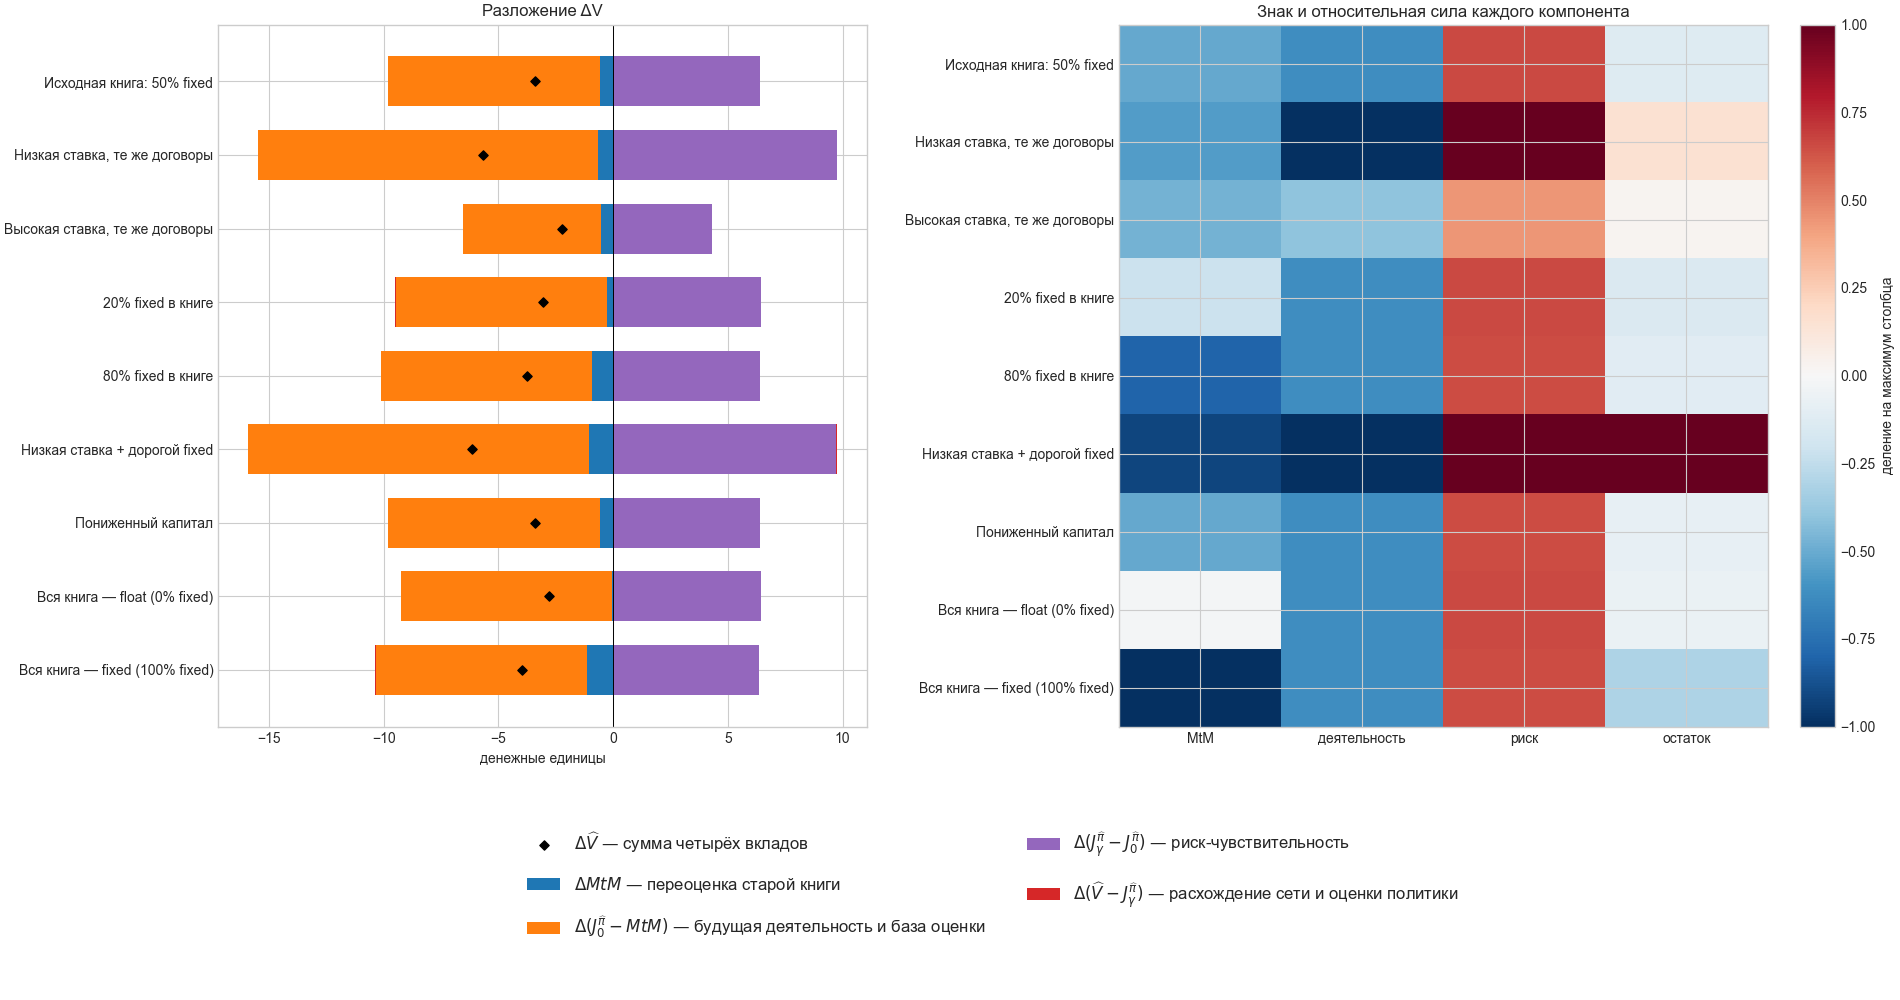
\includegraphics[width=\textwidth,height=.86\textheight,keepaspectratio]{figures/risk_18_four.png}
\end{frame}

\begin{frame}{18. Что показывает разложение $\Delta V$}
\small
В исходном состоянии вклады в денежных единицах:
\[
\underbrace{-0.58}_{\Delta\MtM,}
\underbrace{-9.22}_{\text{будущая деятельность,}}
\underbrace{+6.42}_{\text{риск-чувствительность,}}
\underbrace{-0.01}_{\text{остаток}}
\approx -3.39.
\]
\begin{itemize}
\item $\Delta\MtM$ переоценивает старые договоры; будущая выдача в неё не входит.
\item Член $\Delta(J_0^{\widehat\pi}-\MtM)$ включает рост книги,
дисконтирование будущих выплат и различие оценки под $P$ и $Q$.
Отдельный вклад адаптации здесь не выделяется.
\item Положительный риск-член означает, что после шока разница между
риск-чувствительной и риск-нейтральной оценками стала менее отрицательной.
\end{itemize}
\footnotesize
Оценки политик в сохранённом прогоне не достигли критерия сходимости.
Большие взаимно компенсирующиеся вклады пока диагностические.
\end{frame}


\begin{frame}{19. Ставка и выдача fixed}
\centering
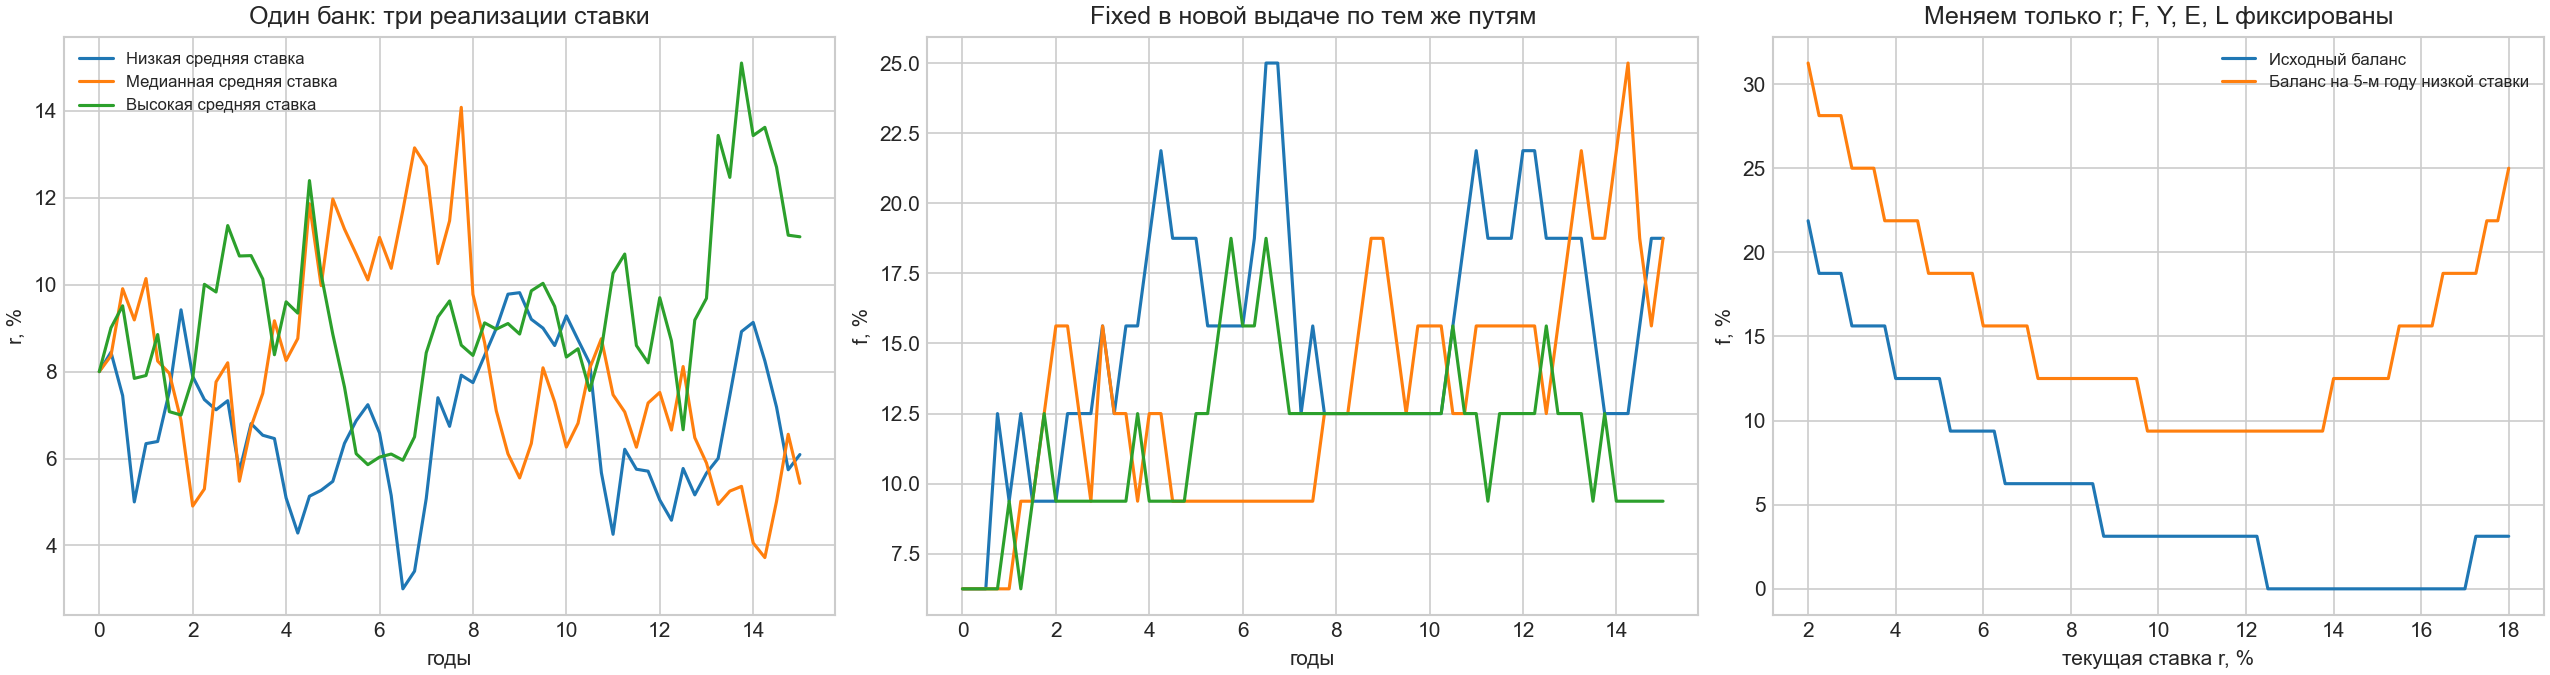
\includegraphics[width=\textwidth,height=.60\textheight,keepaspectratio]{figures/policy_rate_dynamics.png}
\par\smallskip
\begin{minipage}{.96\textwidth}\footnotesize
Две левые панели: три реализации одного банка при $\chi=5$;
вместе со ставкой меняются $F,Y,E,L$.
Справа меняется \emph{только} текущая ставка при фиксированном балансе.
В обычном диапазоне наблюдается обратная зависимость $f$ от $r$,
но при высоких ставках она может разворачиваться.
Ступени отражают численную сетку действий $1/32$.
\end{minipage}
\end{frame}

\begin{frame}{20. Высокий fixed-купон не гарантирует преимущества fixed}
\small
В нашей модели новый fixed-кредит выдаётся с купоном
\[
k_F(r)=\underbrace{A_Q(r)^{-1}-\mu}_{\text{par-купон по всей будущей кривой}}+s_F.
\]
\begin{center}
\begin{tabular}{lrrrr}
\hline
Текущая ставка $r$ & $2\%$ & $8\%$ & $14\%$ & $18\%$\\
Новый fixed-купон $k_F(r)$ & $6.82\%$ & $9.46\%$ & $12.22\%$ & $14.14\%$\\
\hline
\end{tabular}
\end{center}
\begin{itemize}
\item Возврат ставки к среднему уже включён в par-купон.
Прогноз снижения ставки не создаёт бесплатной выгоды от фиксации.
\item При высокой $r$ текущий float-доход может превышать fixed-купон;
при низкой $r$ соотношение обратное. Это объясняет текущий carry,
но само по себе не доказывает оптимальность политики.
\item Решение учитывает весь поток владельцу, старые договоры, фондирование,
спрос на float и риск. Обратная зависимость --- результат данной калибровки,
а не универсальное свойство банковского управления.
\end{itemize}
\end{frame}


\begin{frame}{21. Почему одного уровня купона недостаточно}
\small
Для стоимости на единицу книги $v=V/L$ положим $a=F/L$, $y=Y/L$.
С точностью до членов, не зависящих от $f$, гамильтониан имеет вид
\[
(\mu+g(r))\bigl[fv_a+
 \{fk_F(r)+(1-f)s_V(1-f)\}v_y\bigr].
\]
Его производная по действию пропорциональна
\[
v_a+\{k_F(r)-s_V^0+2\eta(1-f)\}v_y.
\]
\begin{itemize}
\item Рост одного $k_F(r)$ действительно усиливает стимул выдавать fixed:
эта часть интуиции верна.
\item Но вместе со ставкой меняется $v_a/v_y$ --- предельная цена
замены float на fixed относительно дохода по договору.
Она учитывает будущую ставку, фондирование, старую книгу, рост и риск.
\item Поэтому направление изменения $f$ не следует из купона одного кредита.
Это условие непрерывной HJB; расчёт в коде использует конечный Bellman-шаг.
\end{itemize}
\end{frame}



\begin{frame}{22. Риск-аверсия и разложение $\Delta V$}
\centering
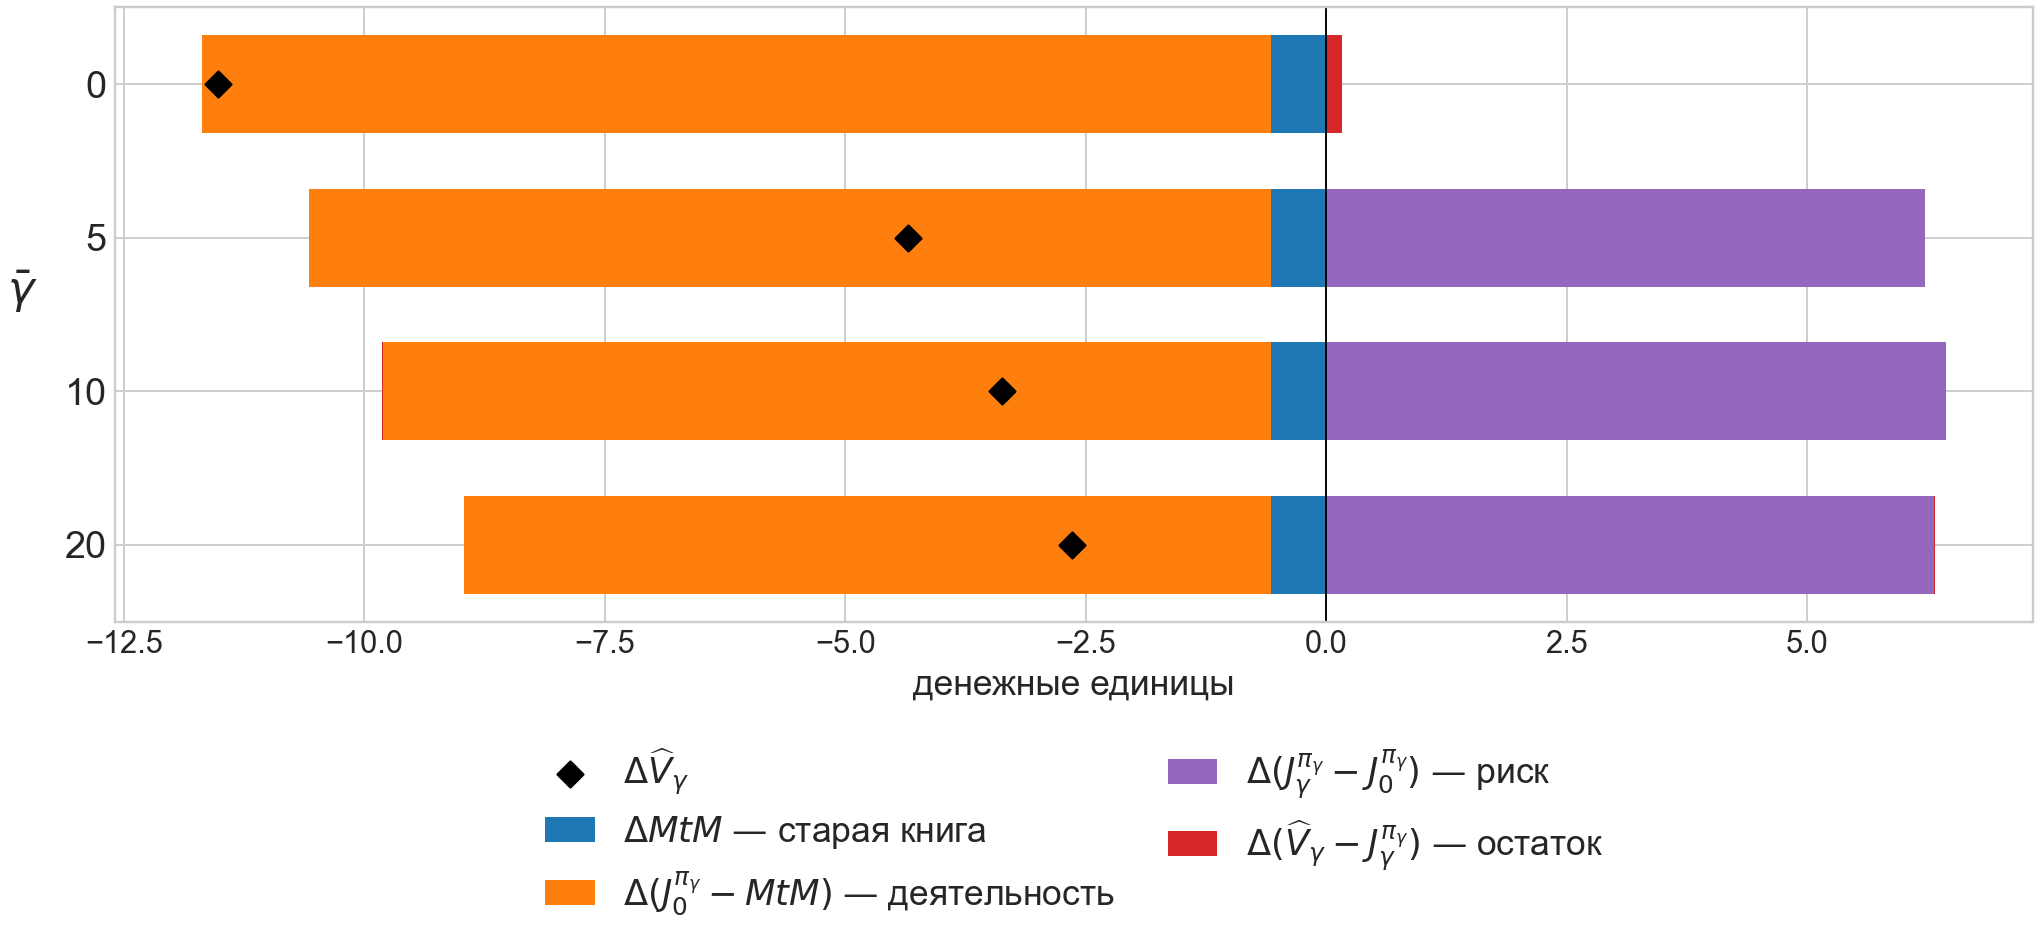
\includegraphics[width=\textwidth,height=.78\textheight,keepaspectratio]{figures/gamma_delta_v_components_slide.png}
\par\vspace{-.5ex}
\begin{minipage}{.97\textwidth}\scriptsize
Одинаковый баланс: $L=100$, $r=8\%$, $F=50$, $Y=5.2304$, $E=12$;
$\eta=0.01$, $\chi=5$. Здесь $\pi_\gamma$ --- сохранённая политика соответствующей gamma.
При $\bar\gamma\ge5$ риск-компонента близка к $+6.2$--$+6.4$;
меняется также стоимость будущей деятельности. Оценки политик не сошлись: размеры вкладов предварительны.
\end{minipage}
\end{frame}

\begin{frame}{23. Влияние gamma на политику и деятельность банка}
\centering
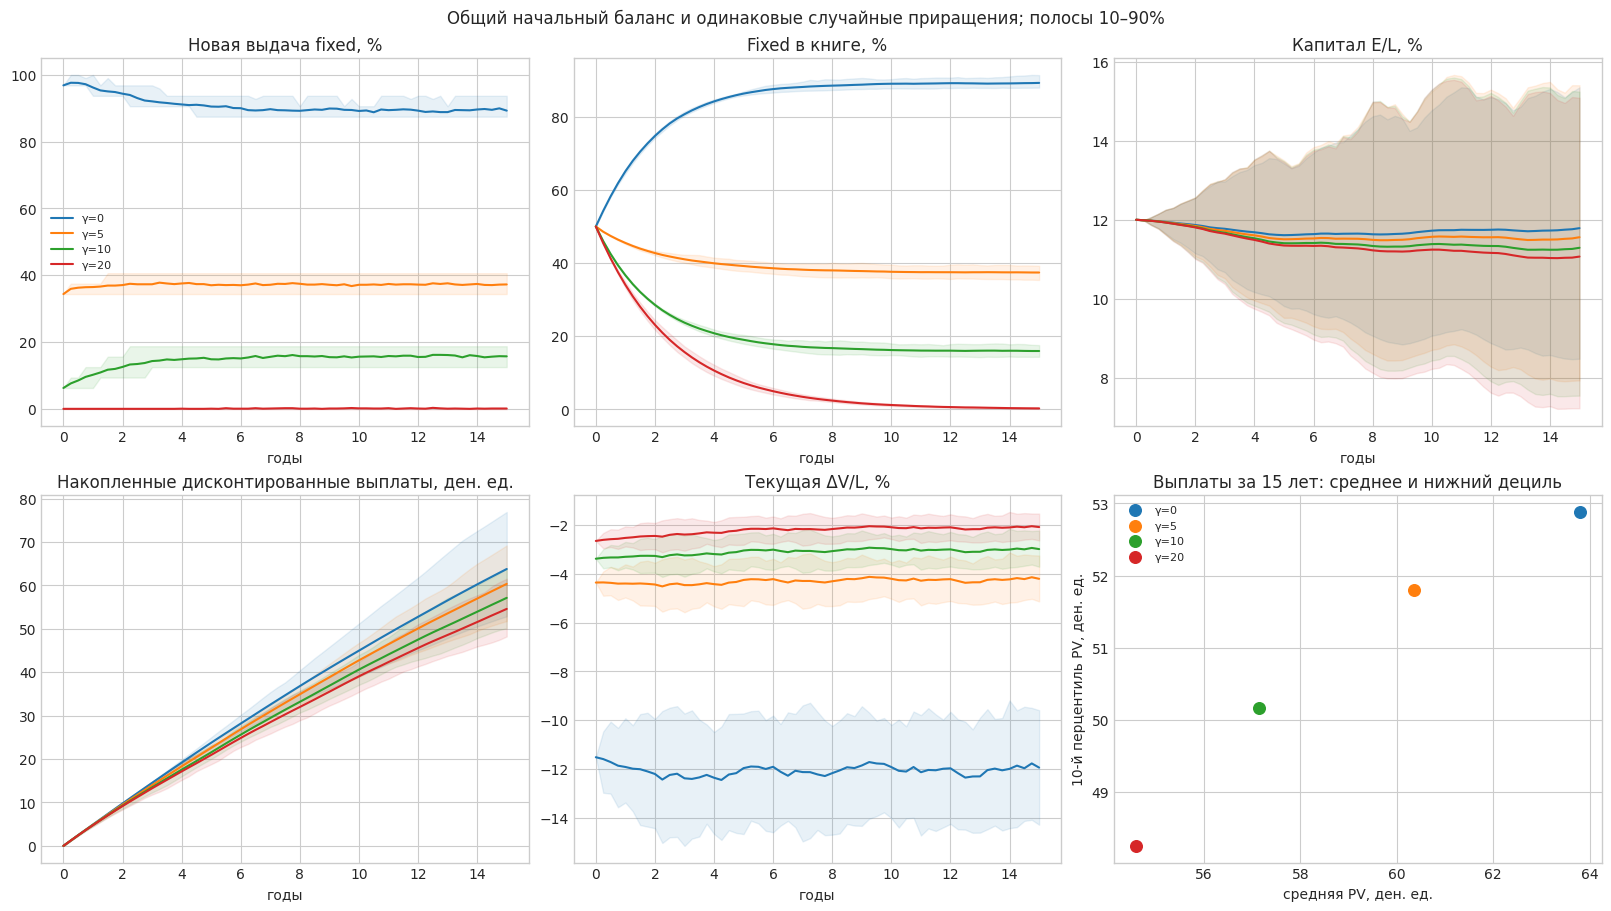
\includegraphics[width=\textwidth,height=.86\textheight,keepaspectratio]{figures/gamma_policy_activity.png}
\par\vspace{-.5ex}
\begin{minipage}{.97\textwidth}\scriptsize
$\eta=0.01$, $\chi=5$. Линии --- среднее, полосы --- 10--90-й перцентили на одинаковых путях ставки.
Большая gamma уменьшает выдачу fixed и средние выплаты в этом прогоне.
Выплаты за 15 лет не равны бессрочному рекурсивному функционалу.
\end{minipage}
\end{frame}

\begin{frame}{24. Временный и перманентный шоки: денежные дельты}
\centering
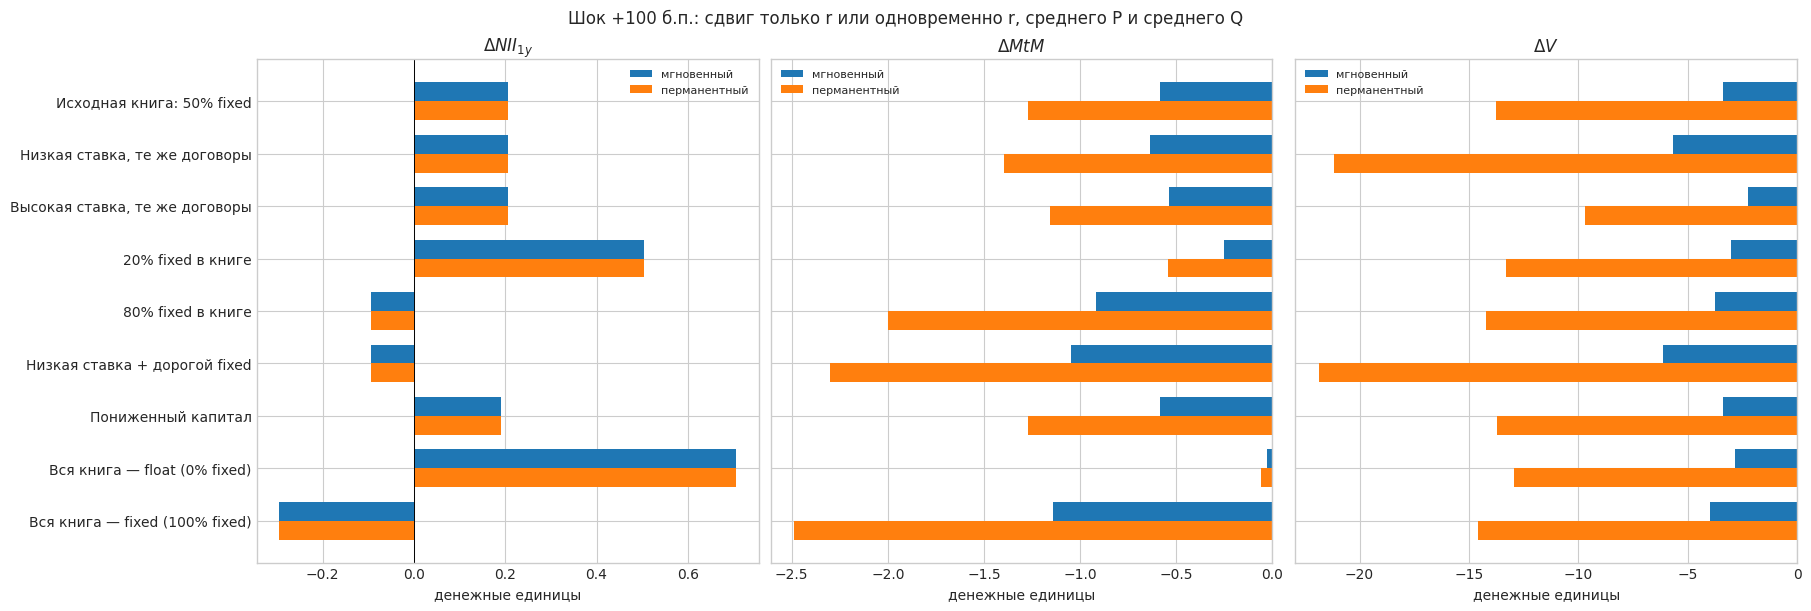
\includegraphics[width=\textwidth,height=.68\textheight,keepaspectratio]{figures/permanent_shock_absolute.png}
\par\smallskip
\begin{minipage}{.97\textwidth}\scriptsize
Отдельный опыт: $\bar\gamma=10$, $\chi=5$; в исходной книге $L=100$, $F=50$, $Y=5.625$, $E=12$.
Временный шок меняет только $r$. Перманентный меняет $r,\bar r_P,\bar r_Q$ на 100 б.п.
В исходном состоянии $\Delta\MtM$: $-0.58\to-1.27$; $\Delta V$: $-3.39\to-13.75$.
Замороженный $\Delta\NII_{1y}$ одинаков: он не использует динамику ставки.
Для V задачи переоптимизированы; обе имеют \texttt{converged=False}, RMSE около 0.007.
\end{minipage}
\end{frame}

\begin{frame}{25. Временный и перманентный шоки: относительные дельты}
\centering
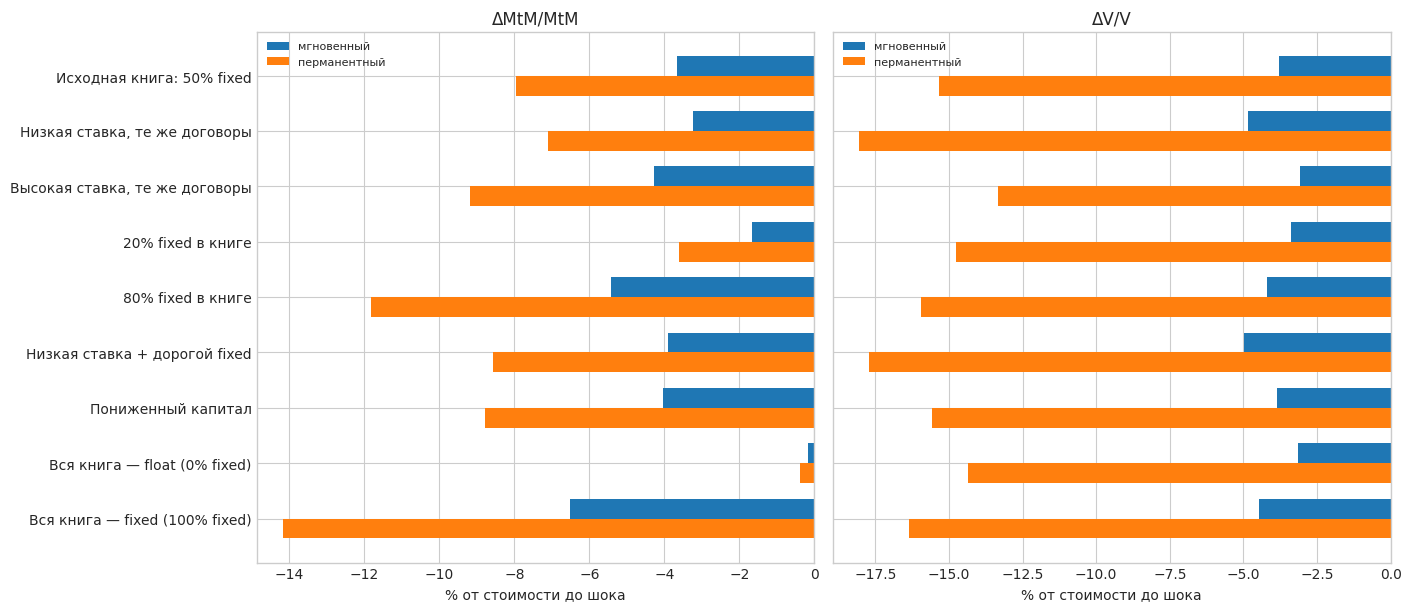
\includegraphics[width=\textwidth,height=.74\textheight,keepaspectratio]{figures/permanent_shock_relative.png}
\par\smallskip
\begin{minipage}{.97\textwidth}\scriptsize
В каждом сценарии два шока делятся на одну и ту же стоимость до шока.
Перманентный сдвиг сильнее меняет и MtM, и V.
В V дополнительно изменяются будущий рост книги, цены новых выдач и денежные потоки,
поскольку сдвинуто также физическое среднее $\bar r_P$.
\end{minipage}
\end{frame}

\begin{frame}{26. Перманентный шок и параллельный сдвиг кривой}
\begin{columns}[T,onlytextwidth]
\begin{column}{.58\textwidth}
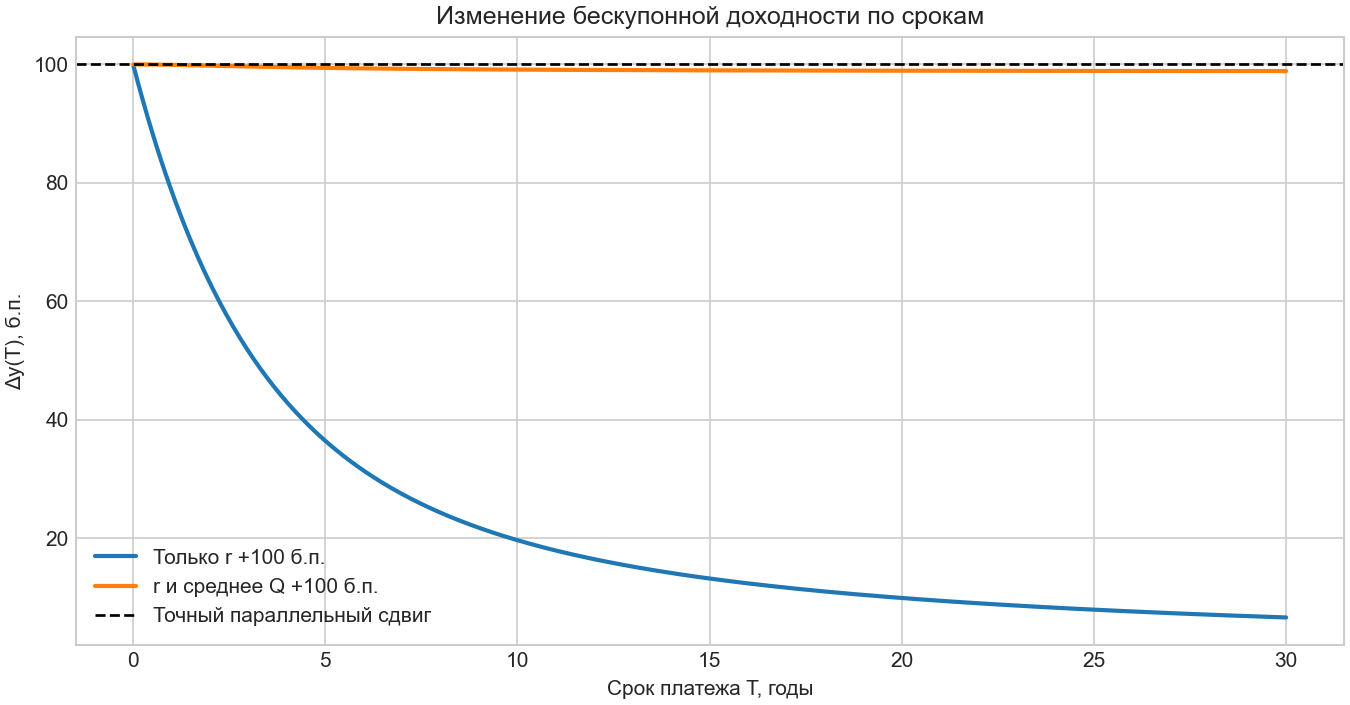
\includegraphics[width=\textwidth]{figures/parallel_curve_comparison.png}
\footnotesize
При исходных $r=\bar r_Q=8\%$.
На коротком конце оба шока равны 100 б.п.; на длинном их эффекты различаются.
\end{column}
\begin{column}{.39\textwidth}\scriptsize
Точный параллельный шок задаётся ценами
\[
P_Q^+(r,T)=e^{-\delta T}P_Q(r,T),
\]
то есть $y^+(T)=y(T)+\delta$ для каждого срока.
\medskip

В CIR повышение $r$ и $\bar r_Q$ --- \textbf{близкий аналог}, но не точное равенство:
волатильность $\sigma\sqrt r$ зависит от уровня.
В нашей калибровке длинная доходность сдвигается примерно на 98.75 б.п.
\medskip

Повышение $\bar r_P$ --- отдельное предположение о будущем режиме экономики.
Оно не следует автоматически из сдвига сегодняшней оценочной кривой.
\end{column}
\end{columns}
\end{frame}

\end{document}

